%%============
%%  ** Author: Shepherd Qirong
%%  ** Date: 2023-04-22 11:36:22
%%  ** Github: https://github.com/ShepherdQR
%%  ** LastEditors: Shepherd Qirong
%%  ** LastEditTime: 2023-04-22 12:27:31
%%  ** Copyright (c) 2019--20xx Shepherd Qirong. All rights reserved.
%%============



\documentclass[UTF8]{../../../../RepresentationUniverse}
\begin{document}

\title{How Things Work}
\date{Created on 20230422.\\   Last modified on \today.}
\maketitle
\tableofcontents

\chapter{Introduction}

Discovery Science, How Things Work. 10 episodes.

\begin{figure}[h]
    \centering
    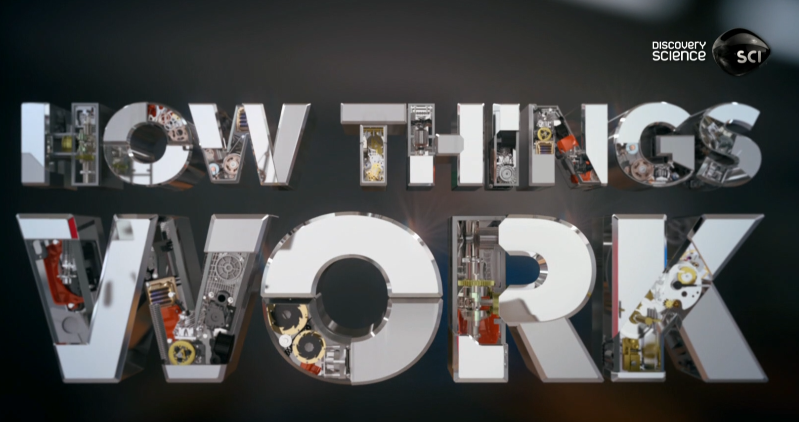
\includegraphics[width=0.5\textwidth]{./src/figures/Cover-Snipaste_2023-04-22_11-38-06.png}
    \caption{[Discovery Science, How Things Work]}
    \label{figure:How Things Work}
\end{figure}



\chapter{Ep1}

\section{chainSaw}

链条转动环绕的锯面,坚韧、轻盈,是两层铁片中间有夹层。

链条有3排镀铬的刀片。

引擎:单杠。关键是曲轴。火烧6小时,一次烧2500个。

测试:机器模拟人工。

保护:上翘反弹时,抓手前护垫压迫停机。

减震性。

\begin{figure}[h]
    \centering
    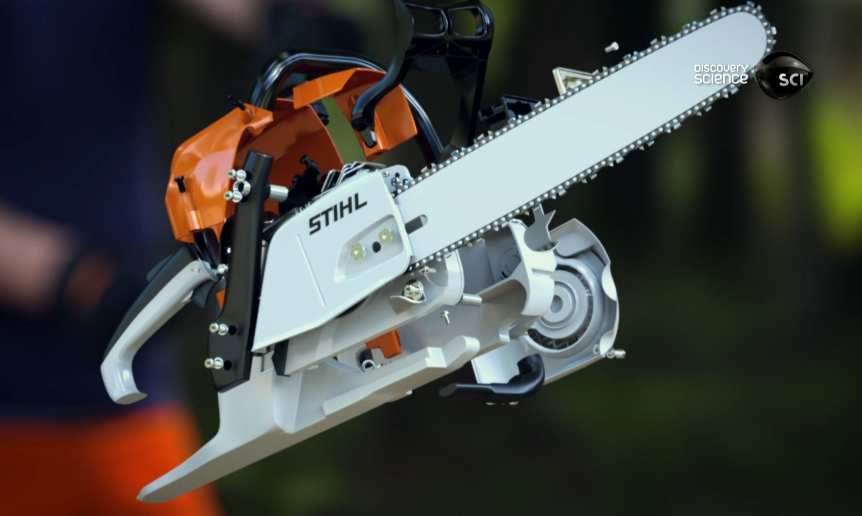
\includegraphics[width=0.5\textwidth]{./src/figures/chainSaw-Snipaste_2023-04-22_11-42-32.png}
    \caption{[chainSaw]}
    \label{figure:chainSaw}
\end{figure}


\section{jukebox}

复古音色:木质机箱,弯曲木片并粘贴。5个喇叭。

换片:二轴,夹取唱片。

外观:弯曲的玻璃,其中有泡泡。 

\begin{figure}[h]
    \centering
    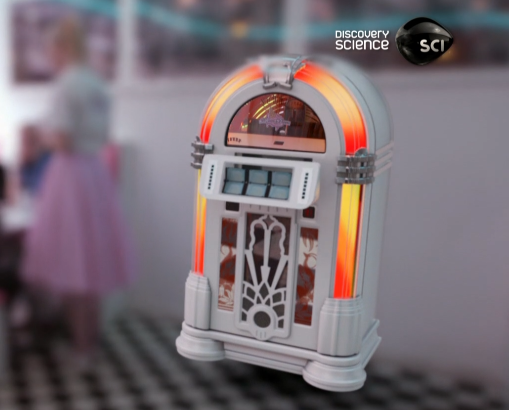
\includegraphics[width=0.5\textwidth]{./src/figures/jukebox_2023-04-22_11-52-45.png}
    \caption{[jukebox]}
    \label{figure:jukebox}
\end{figure}


\section{FishingReel}

实心铝柱体掏出骨架。氧化并上色,防腐蚀。

制动器,手工组装141个零件。


\begin{figure}[h]
    \centering
    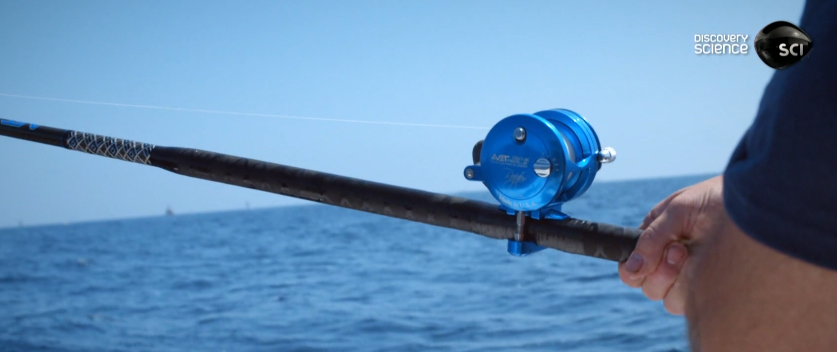
\includegraphics[width=0.5\textwidth]{./src/figures/FishingReel_2023-04-22_11-58-00.png}
    \caption{[FishingReel]}
    \label{figure:FishingReel}
\end{figure}

\begin{figure}[h]
    \centering
    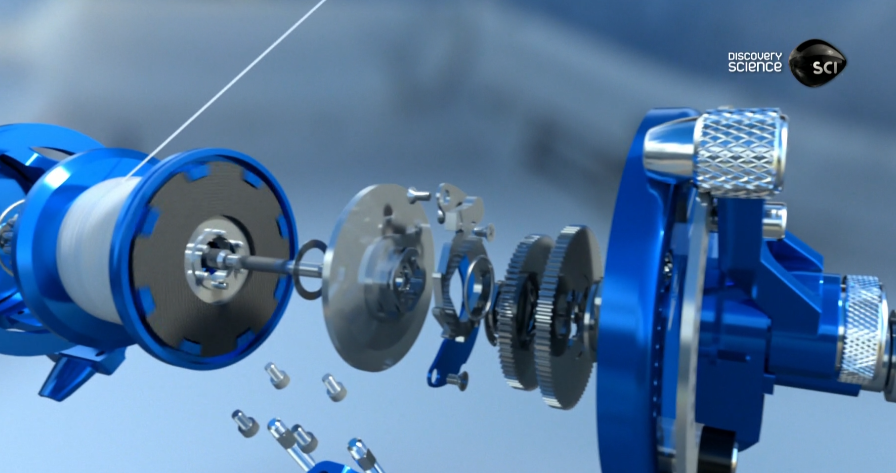
\includegraphics[width=0.5\textwidth]{./src/figures/FishingReel02_2023-04-22_11-58-00.png}
    \caption{[FishingReel02]}
    \label{figure:FishingReel02}
\end{figure}


\section{CarWash}

1000多零件。

龙门架。

传送带: 可运送2吨。

刷子:软布。高转速。不刮伤车,不粘连。

喷水,泡沫。

烘干:高转速,扭矩扳手保证安全可靠。

\begin{figure}[h]
    \centering
    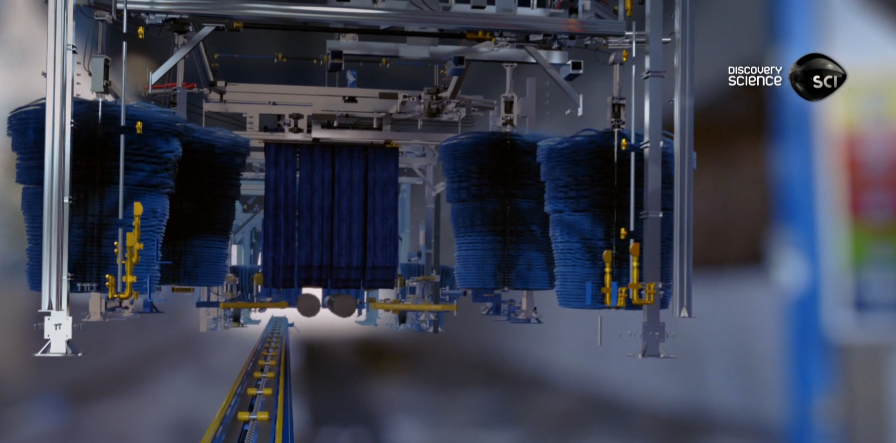
\includegraphics[width=0.5\textwidth]{./src/figures/CarWash_2023-04-22_12-04-43.png}
    \caption{[CarWash]}
    \label{figure:CarWash}
\end{figure}

\begin{figure}[h]
    \centering
    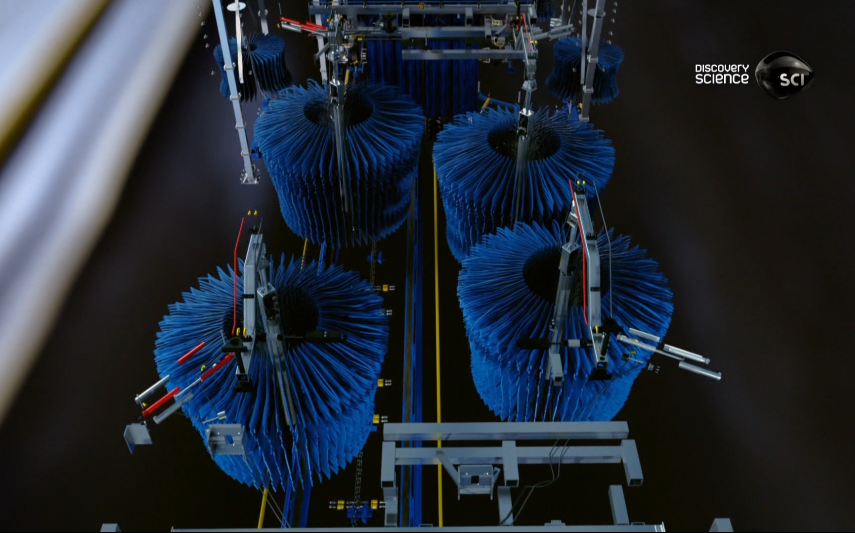
\includegraphics[width=0.5\textwidth]{./src/figures/CarWash02_20230422_120921.png}
    \caption{[CarWash02]}
    \label{figure:CarWash02}
\end{figure}


\section{Juicer}

外壳:注塑、透明,有5个面,其中有1个小面。

马达:1s300转。

驱动轴,轴两端有轴承。

刀片

防漏:特氟龙垫圈包裹轴承

\begin{figure}[h]
    \centering
    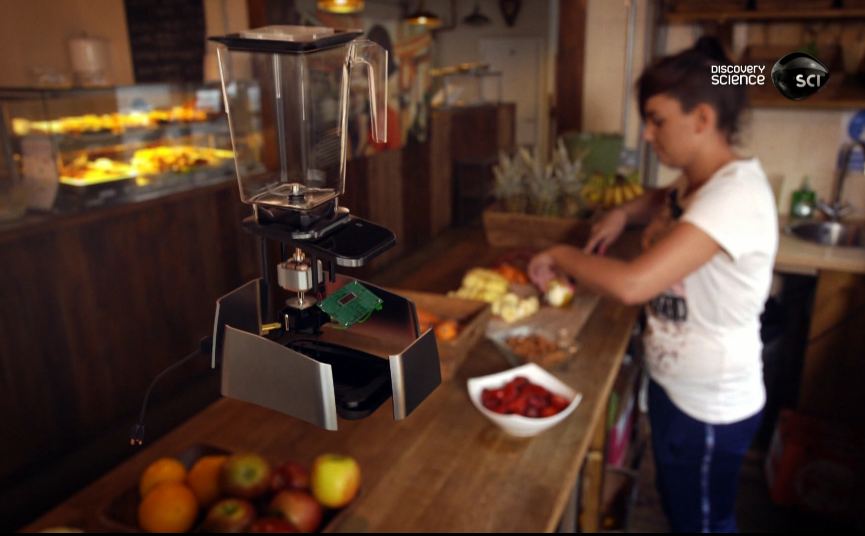
\includegraphics[width=0.5\textwidth]{./src/figures/Juicer_20230422_121257.png}
    \caption{[Juicer]}
    \label{figure:Juicer}
\end{figure}




\section{BikePump}

手工组装74个零件。 

单向阀。皮革塞和内壁镗到镜面光洁的管。

\begin{figure}[h]
    \centering
    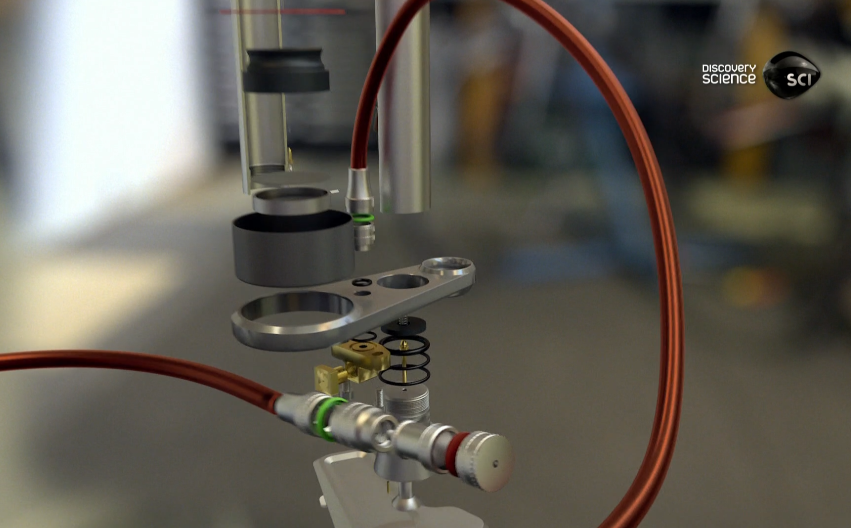
\includegraphics[width=0.5\textwidth]{./src/figures/BikePump_20230422_122128.png}
    \caption{[BikePump]}
    \label{figure:BikePump}
\end{figure}


压力表:压力使鼓膜向上鼓起,压缩弹簧,弹簧旋转转化为指针。
\begin{figure}[h]
    \centering
    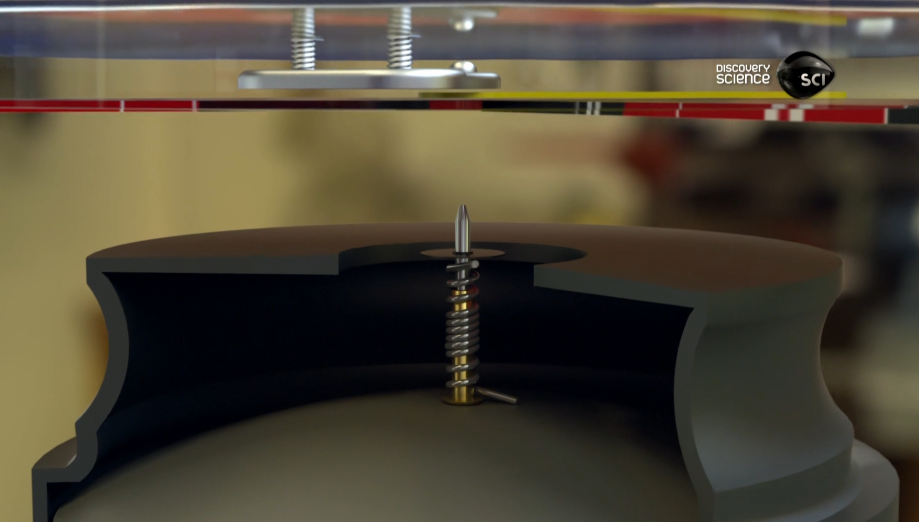
\includegraphics[width=0.5\textwidth]{./src/figures/BikePump02_20230422_122432.png}
    \caption{[BikePump02]}
    \label{figure:BikePump02}
\end{figure}


\end{document}